% !TEX root = ../../beamer/ba_beamer_master.tex
% @author Marcel Ruland (2018)
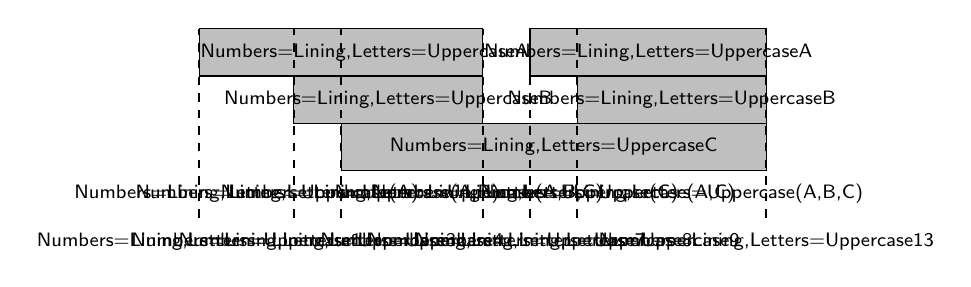
\begin{tikzpicture}[
	scale=0.6,
	every node/.append style={font=\scriptsize\sffamily\addfontfeature{Numbers=Lining,Letters=Uppercase}}]
	% boxes
	\draw [fill=lightgray] (0,4) rectangle (6,5);  % A1
	\node at (3.5,4.5) {A};
	
	\draw [fill=lightgray] (7,4) rectangle (12,5);  % A2
	\node at (9.5,4.5) {A};
	
	\draw [fill=lightgray] (2,3) rectangle (6,4);  % B1
	\node at (4,3.5) {B};
	
	\draw [fill=lightgray] (8,3) rectangle (12,4);  % B2
	\node at (10,3.5) {B};
	
	\draw [fill=lightgray] (3,2) rectangle (12,3);  % C
	\node at (7.5,2.5) {C};
	
	% item sets
	\node at (1,1.5) {(A)};
	\node at (2.5,1.5) {(A,B)};
	\node at (4.5,1.5) {(A,B,C)};
	\node at (6.5,1.5) {(C)};
	\node at (7.5,1.5) {(A,C)};
	\node at (10,1.5) {(A,B,C)};
	
	% time points
	\node at (0,0.5) {1};
	\node at (2,0.5) {3};
	\node at (3,0.5) {4};
	\node at (6,0.5) {7};
	\node at (7,0.5) {8};
	\node at (8,0.5) {9};
	\node at (12,0.5) {13};
	
	% time point lines
	\draw [dashed, thick] (0,1) -- (0,5);
	\draw [dashed, thick] (2,1) -- (2,5);
	\draw [dashed, thick] (3,1) -- (3,5);
	\draw [dashed, thick] (6,1) -- (6,5);
	\draw [dashed, thick] (7,1) -- (7,5);
	\draw [dashed, thick] (8,1) -- (8,5);
	\draw [dashed, thick] (12,1) -- (12,5);
\end{tikzpicture}